\section{Layer~2 – From Isolated Dots to a Web of Relations}
\label{sec:layer2}

% ----- SUPERKRACHT -----
\begin{tcolorbox}[colback=blue!5, colframe=blue!60, title=\textbf{Superpower: The Networker}]
\begin{center}
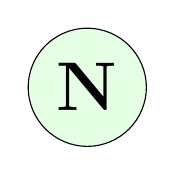
\begin{tikzpicture}
  \node[draw, circle, fill=green!10, minimum size=1.5cm, font=\bfseries\Huge] {N};
\end{tikzpicture}
\textit{“Who talks to whom?”}
\end{center}
\end{tcolorbox}

One atom alone is useless.  It’s like a single word spoken in an empty
room – it has no context, no connection.  Meaning only emerges when
atoms start talking to each other.

\begin{tcolorbox}[colback=yellow!5, colframe=yellow!80, title=Real‑life analogy]
Look at the night sky.  Every star is a lonely point of light.  But
your brain connects them with imaginary lines and sees a bear, a
hunter, a swan.  Those constellations do not exist “out there”; they
exist in the relationships \emph{between} the stars.

Pixel does exactly this with pixels.  A single bright pixel is a star;
when many bright pixels appear close together, Pixel draws a web of
connections between them.  Over time, this web becomes a map of the
world — a \textbf{hypergraph} — that tells Pixel which stars belong to
the same constellation.
\end{tcolorbox}

\textbf{Pixel’s journey continues.}
After many snapshots of the Martian landscape, Pixel notices something:
bright pixels near the horizon often fire together with dark pixels
right next to them.  A strong connection appears.  Other pixel‑pairs
barely ever co‑activate – a weak connection.  Pixel begins to draw a
giant map where every dot is linked to others with a number that says
how tightly they belong together.

\begin{figure}[ht]
\centering
\begin{tikzpicture}[
    node/.style={circle, draw=black, fill=blue!5, minimum size=0.7cm},
    edge/.style={-{Stealth}, thick, color=gray}
]
\node[node] (a) at (0,0) {A};
\node[node] (b) at (2,1) {B};
\node[node] (c) at (4,0) {C};
\node[node] (d) at (2,-1){D};
\draw[edge] (a) -- node[above left] {0.8} (b);
\draw[edge] (b) -- node[above right]{0.6} (c);
\draw[edge] (c) -- node[below right]{0.9} (d);
\draw[edge] (d) -- node[below left] {0.3} (a);
\draw[edge] (a) -- node[above] {0.1} (c);
\draw[edge] (b) -- node[right] {0.4} (d);
\node at (2,-2) {\small Pixel’s first social network of pixels};
\end{tikzpicture}
\caption{Four observables linked by weighted connections.}
\label{fig:network}
\end{figure}

This map is called a \textbf{hypergraph} – a web of relationships that
will later tell Pixel where to look for interesting structures.  Notice
that Pixel still does not know what a “rock” is; it only senses who
co‑occurs with whom.  That is the first, crucial break away from
human‑centered thinking.

\subsection*{Why a hypergraph and not just a simple network?}

In an ordinary social network, you can only be friends with
individuals.  But in the real world, a group of three stars might form
a triangle that has a special meaning.  A hypergraph allows Pixel to
record not only “A talks to B”, but also “A, B, and C light up
simultaneously”.  This ability to see groups, not just pairs, is what
makes the hypergraph such a powerful discovery tool.

\begin{tcolorbox}[colback=blue!5, colframe=blue!40, title=Try this at home]
Open a photo on your phone and zoom all the way in.
Do you see how a patch of sky is made of thousands of tiny squares
that all have very similar colours?  Those squares are strongly
connected in Pixel’s hypergraph — they are his “Milky Way”.
\end{tcolorbox}

% ----- WAT ALS...? -----
\begin{tcolorbox}[colback=orange!5, colframe=orange!60, title=\textbf{What if...?}]
What if Pixel only had one picture to learn from?  Could it still
discover meaningful constellations, or would it be like trying to draw
a map of the sky after seeing only one star?
\end{tcolorbox}